\section{Results and Discussion}
\label{sec:results}

\subsection{Dual-view model trained at the reported 10K scale}

We developed a dual-view detector that combines image context with native-resolution crop evidence. The 10K run summary records 10,000 training images, 15,000 steps, a global batch of 16, and two Tesla T4 GPUs. It describes inference with multi-scale tiles and flip augmentation. Table~\ref{tab:10k-summary} records the aggregate results supplied for this run and the values available from the common OpenSDID evaluation in FUSED~\cite{fused}. The earlier 100-image ensemble evaluation remains a separate development result.

\begin{table*}[t]
\centering\small
\caption{Literature benchmark values and the reported 10K run summary, in percent. The literature columns use FUSED's SD1.5-only protocol. A dash indicates a value unavailable in its main OpenSDID tables. The 10K column is transcribed from the run summary. Aggregate detection metrics require reconciliation with the accompanying counts. $^{\dagger}$FUSED reports per-image pixel F1; the 10K aggregation is undocumented, so these values are not directly comparable.}
\label{tab:10k-summary}
\begin{tabular}{@{}lrrrrr@{}}
\toprule
Metric & TruFor & DeCLIP & MaskCLIP & FUSED & 10K dual-view model \\
\midrule
Image accuracy & 69.80 & 73.10 & 82.00 & 89.50 & 91.20 \\
Balanced accuracy & -- & -- & -- & -- & 92.60 \\
Image F1 & 58.60 & 71.40 & 77.80 & 88.00 & 89.60 \\
Image AUROC & -- & -- & -- & -- & 93.40 \\
Genuine specificity & -- & -- & -- & -- & 94.00 \\
Image false-positive rate & -- & -- & -- & -- & 6.00 \\
Mean localization IoU & 36.90 & 25.20 & 42.70 & 44.50 & 47.30 \\
Localization pixel F1$^{\dagger}$ & 42.60 & 30.30 & 49.40 & 55.30 & 63.80 \\
SD1.5 IoU & 63.40 & 37.20 & 67.10 & 59.60 & 68.40 \\
SD2.1 IoU & 54.70 & 35.70 & 55.50 & 52.40 & 56.10 \\
SD3 IoU & 32.30 & 27.30 & 43.80 & 50.00 & 52.70 \\
SDXL IoU & 26.60 & 14.60 & 31.00 & 37.50 & 41.80 \\
FLUX.1 IoU & 7.60 & 11.20 & 16.20 & 22.90 & 29.50 \\
Tiny-edit IoU (below 2\%) & -- & -- & -- & -- & 13.60 \\
Medium-edit IoU (2--10\%) & -- & -- & -- & -- & 38.50 \\
Large-edit IoU (above 10\%) & -- & -- & -- & -- & 54.20 \\
\bottomrule
\end{tabular}
\end{table*}

The reported 10K model exceeds FUSED's published OpenSDID scores by 1.70 percentage points in image accuracy (91.20\% versus 89.50\%) and 2.80 points in mean localization IoU (47.30\% versus 44.50\%). These numerical differences compare the Gemini run summary with the published benchmark. The training protocols differ.

The supplied confusion counts are 46 true positives, 47 true negatives, three false positives and four false negatives. They imply 93.0\% accuracy, 93.0\% balanced accuracy and 92.93\% edited-class F1 for those 100 predictions. Specificity and false-positive rate agree with the table. The reported aggregate IoU of 47.30\% also differs from the unweighted mean of the five reported editor IoUs (49.70\%). Per-image predictions and aggregation rules are needed to resolve these discrepancies and establish a matched comparison with prior methods.

\begin{figure}[t]
\centering
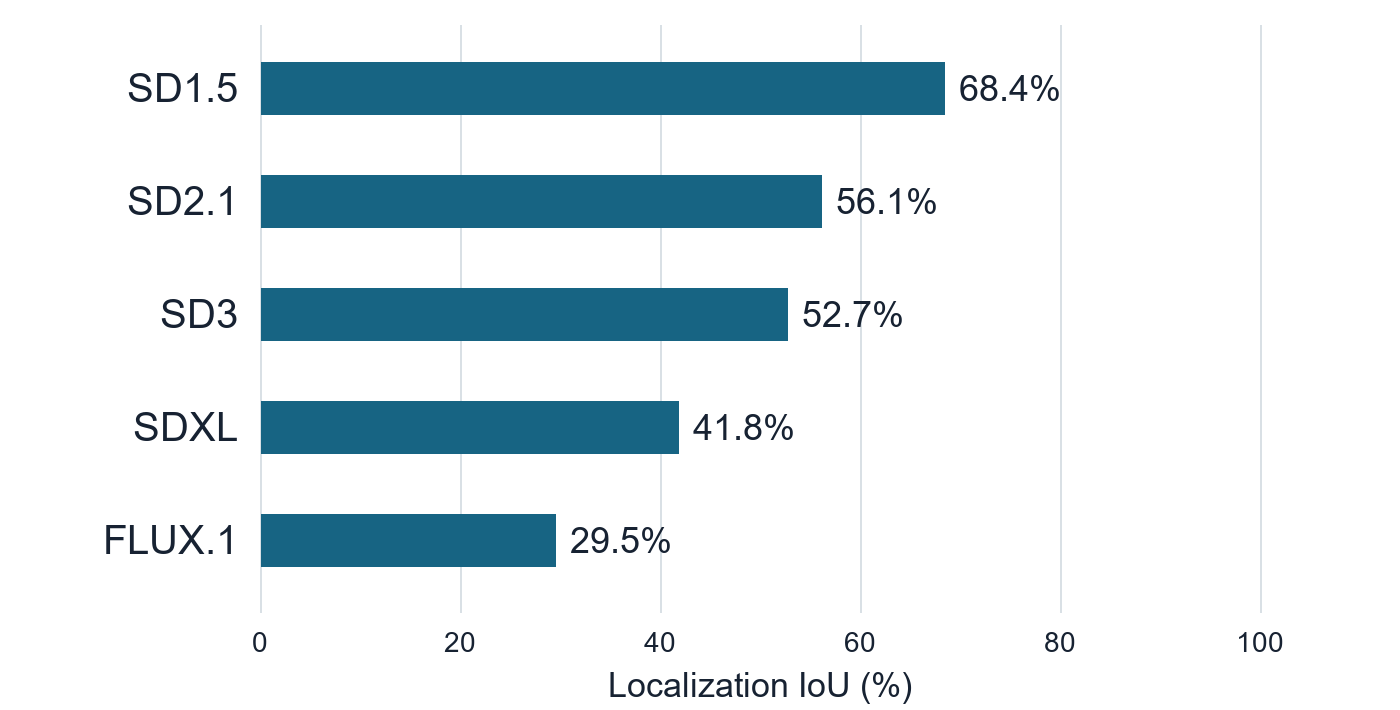
\includegraphics[width=\columnwidth]{figures/10k-editor-iou.png}
\caption{Per-editor localization IoU transcribed from the 10K run summary. Values are shown by editor so the variation across generators remains visible.}
\Description{Horizontal bars show SD1.5 68.4, SD2.1 56.1, SD3 52.7, SDXL 41.8 and FLUX.1 29.5 percent IoU.}
\label{fig:10k-editors}
\end{figure}

Figure~\ref{fig:10k-editors} shows the strongest reported overlap on SD1.5 and the weakest on FLUX.1. The edit-size rows show a similar spread, from 13.60\% for tiny edits to 54.20\% for large edits. Both breakdowns are useful for identifying where to inspect predictions once the run artifacts are available.
\subsection{Dataset and evaluation protocol}
\label{sec:experiments}

We use a 100-image development subset drawn from OpenSDID~\cite{opensdi}. The subset includes 20 images per editor group (SD~1.5, SD~2.1, SDXL, SD~3, and FLUX.1), split evenly between genuine and edited images within each group. The subset has been inspected during development. We use it to compare available checkpoints and diagnose errors. An independent evaluation on source-disjoint images remains pending.

We report image accuracy, edited-class F1, and area under the receiver operating characteristic curve (AUROC). For localization, mean intersection over union (IoU) gives each edited image equal weight. We also report IoU by edited area as a proportion of the image and pixel F1 pooled across edited images. Pooling pixels gives large masks more influence than averaging the F1 of each image. For the ensemble, the saved evaluation applies an image-score threshold of 0.9358 and a mask threshold of 0.35. The image threshold was reused from an earlier configuration, so the reported operating point remains exploratory.

\subsection{Image-level detection}

Table~\ref{tab:development-detection} compares checkpoints using their recorded scoring configurations. The ensemble classified 70 of 100 images correctly. The joint-view model had fewer false alarms than the earlier Base whole-image head, with 8 versus 13 genuine images flagged. It also missed 33 edits, compared with 23 for the earlier head. Its accuracy fell from 64\% to 59\%. This tradeoff motivates comparing recall at matched false-positive rates and inspecting the missed edits by size and editor.

\begin{table}[t]
\caption{Image-level detection on the 100-image development subset. Scores are percentages except AUROC. The training and scoring configurations differ across rows.}
\label{tab:development-detection}
\centering
\small
\begin{tabular}{@{}lrrr@{}}
\toprule
Configuration & Acc. & F1 & AUROC \\
\midrule
Small, whole image & 64.0 & 63.27 & 0.6836 \\
Base, whole image & 64.0 & 60.00 & 0.6872 \\
Scaled pilot, combined score & 65.0 & 61.54 & 0.6700 \\
Joint view, whole image & 59.0 & 45.33 & 0.6450 \\
Two-model ensemble & 70.0 & 62.50 & 0.7452 \\
\bottomrule
\end{tabular}
\end{table}

\subsection{Localization across editors and edit sizes}

The ensemble obtained 34.89\% mean IoU and 58.30\% pooled pixel F1. Mean IoU was 8.94\% for edits occupying less than 2\% of an image, 29.33\% for the 2--10\% bin, and 45.16\% for edits larger than 10\%. The small-edit result shows that localization deteriorates when the altered region occupies little of the frame. Table~\ref{tab:development-editor} provides the editor breakdown. SDXL was the weakest group for detection by accuracy and AUROC in this run. Each accuracy estimate represents only 20 images, so a single prediction changes the estimate by five percentage points.

\begin{table}[t]
\caption{Ensemble results by editor group on the development subset. Accuracy and IoU are percentages. Each group contains ten genuine images and ten edited images. IoU is averaged over edited images.}
\label{tab:development-editor}
\centering
\small
\begin{tabular}{@{}lrrr@{}}
\toprule
Editor group & Acc. & AUROC & IoU \\
\midrule
SD~1.5 & 75.0 & 0.9000 & 55.03 \\
SD~2.1 & 70.0 & 0.7100 & 35.84 \\
SDXL & 60.0 & 0.5600 & 24.57 \\
SD~3 & 70.0 & 0.8700 & 33.43 \\
FLUX.1 & 75.0 & 0.7100 & 25.58 \\
\bottomrule
\end{tabular}
\end{table}

\subsection{How the development metrics are computed}

Let TP, TN, FP, and FN denote counts at the chosen image threshold. We compute image accuracy as $(\mathrm{TP}+\mathrm{TN})/N$ and edited-class F1 as $2\mathrm{TP}/(2\mathrm{TP}+\mathrm{FP}+\mathrm{FN})$. AUROC uses the continuous image scores. The localization IoU for an edited image is $|P\cap G|/|P\cup G|$, where $P$ is the predicted mask and $G$ is its reference. We average this quantity over edited images and report the same average within each size bin. An image false alarm counts one genuine image flagged as edited. Predicted mask area on genuine images measures a different kind of error and is reported separately when available.

\subsection{What changes across editors and edit sizes}

Figure~\ref{fig:editor-results} shows that editor rankings differ between image classification and localization. For example, FLUX.1 and SD1.5 both reach 75\% image accuracy, while mean IoU differs by 29.45 percentage points. Detecting an altered image is therefore insufficient evidence that the model has identified the edit correctly. The size stratification in Figure~\ref{fig:size-iou} points to a separate localization bottleneck. Tiny regions have fewer pixels available to support a coherent prediction, and an off-target prediction can dominate the union in IoU.

\begin{figure}[t]
\centering
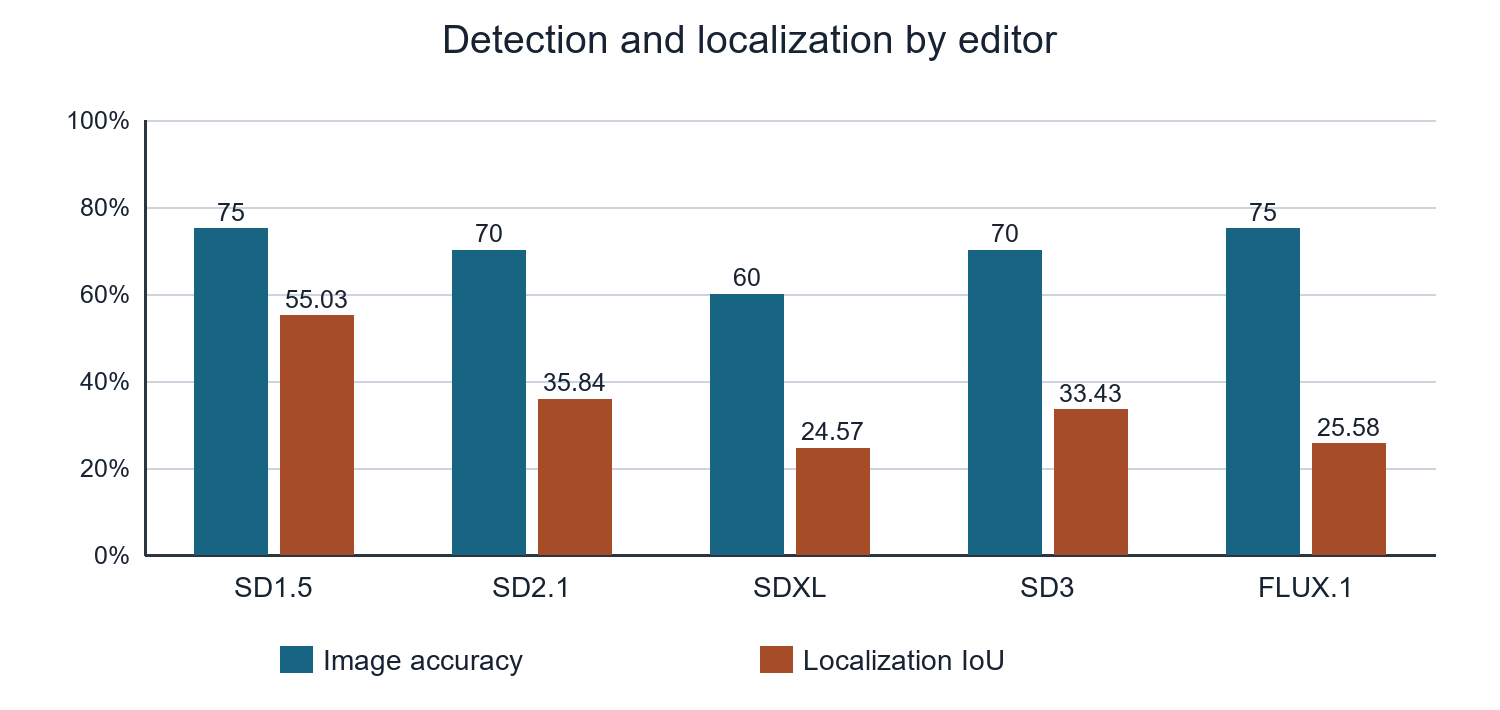
\includegraphics[width=\columnwidth]{figures/editor-results.png}
\caption{Ensemble image accuracy and mean localization IoU on the five editor groups. Each accuracy estimate uses 20 images and each IoU estimate uses the ten edited images in that group.}
\Description{A grouped bar chart of image accuracy and localization overlap for five editors.}
\label{fig:editor-results}
\end{figure}

\begin{figure}[t]
\centering
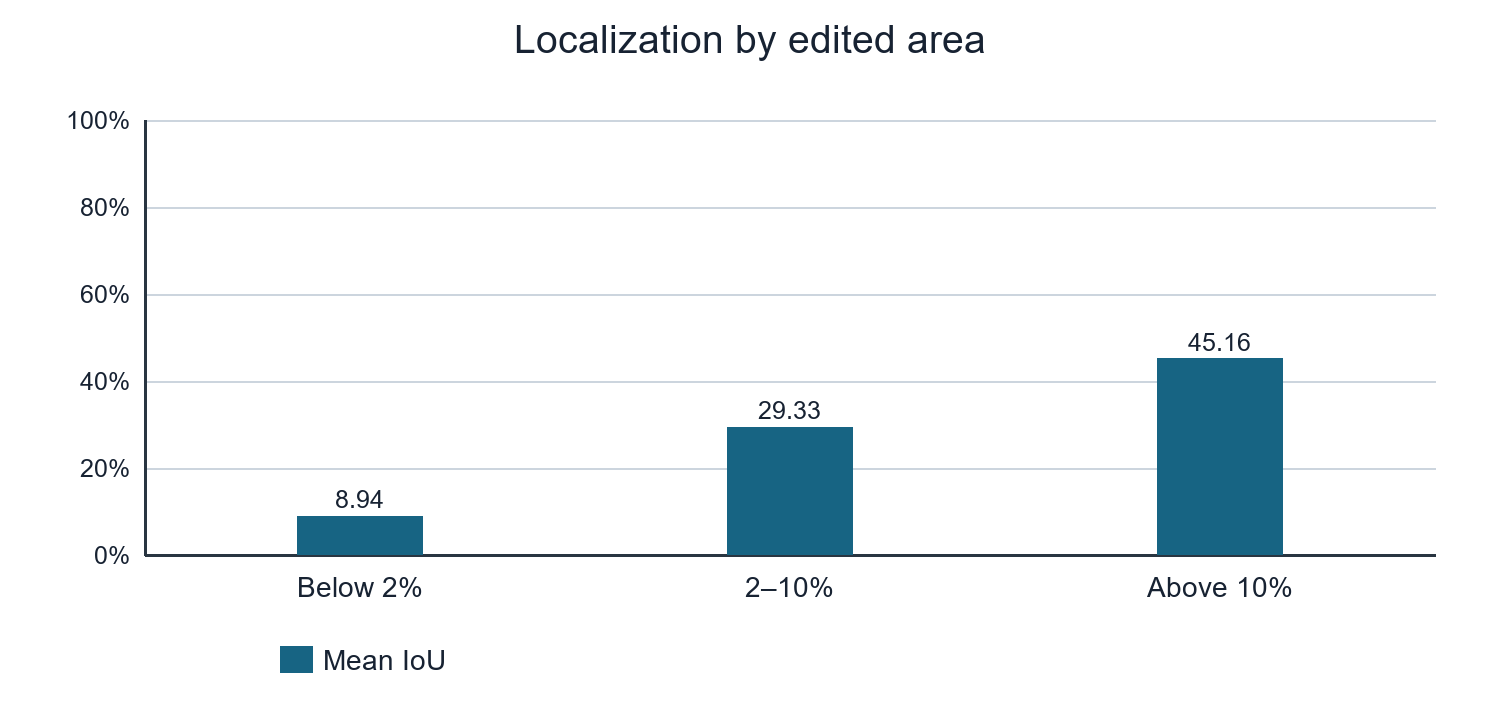
\includegraphics[width=\columnwidth]{figures/edit-size-iou.png}
\caption{Ensemble mean IoU grouped by annotated edit area. The area bins use the reference masks.}
\Description{Three bars show increasing mean overlap as edit area increases.}
\label{fig:size-iou}
\end{figure}

\subsection{The cost of fewer false alarms}

The two whole-image decisions in Figure~\ref{fig:decision-errors} both use 50 genuine and 50 edited images. The joint-view model reduced the false-positive rate from 26\% to 16\%, while edited-image recall fell from 54\% to 34\%. Each row uses its own validation-selected threshold. To distinguish a threshold effect from a better detector, a follow-up experiment should compare both models at a common false-positive rate on fresh data.

\begin{figure}[t]
\centering
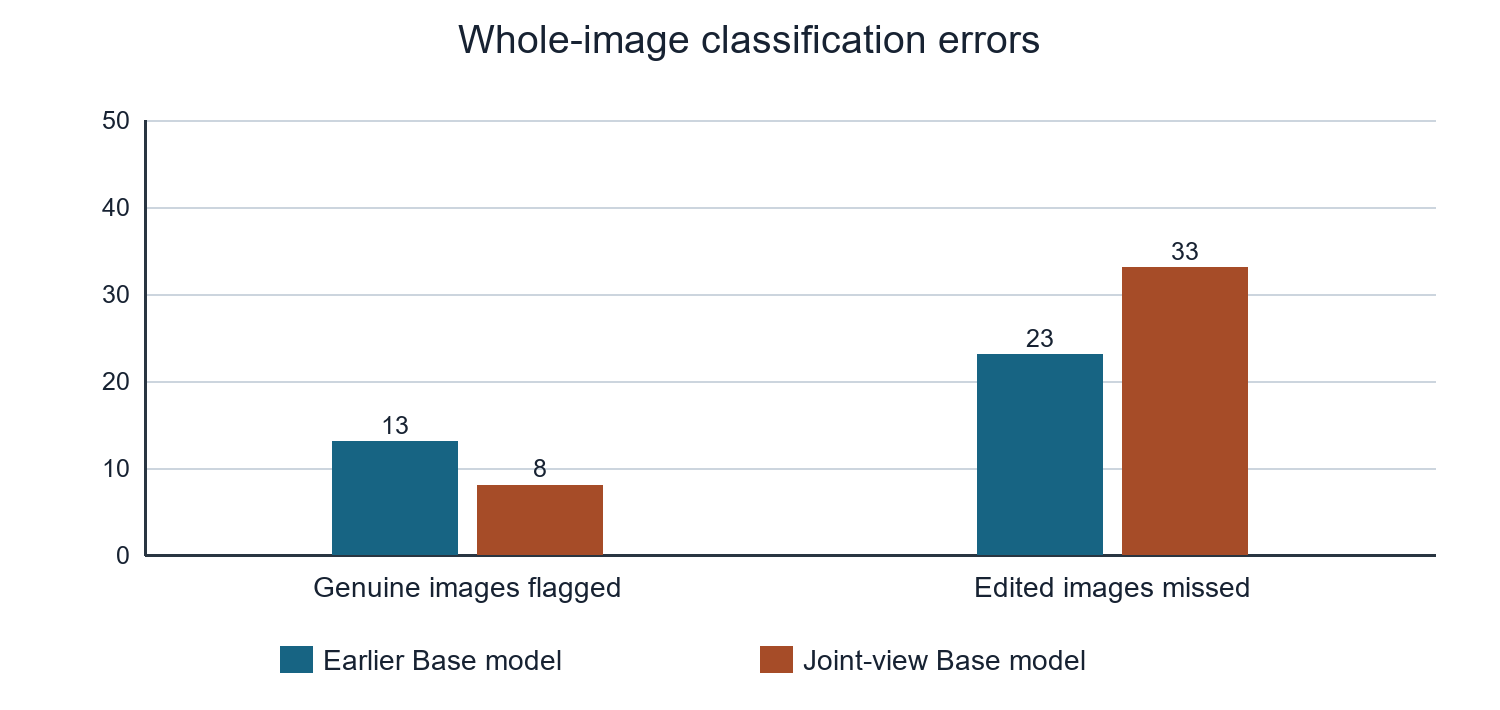
\includegraphics[width=\columnwidth]{figures/decision-errors.png}
\caption{False alarms and missed edits for the earlier and joint-view Base whole-image classifiers. These are counts at their respective operating points on the same development images.}
\Description{Grouped bars show eight versus thirteen false alarms and thirty-three versus twenty-three missed edits for joint-view and earlier Base classifiers.}
\label{fig:decision-errors}
\end{figure}

\subsection{Tile selection under a limited inspection budget}

We also ran a small validation pilot with a maximum of four tiles from a nine-position grid. Selecting tiles based on the whole-image heatmap yielded 35.80\% mean IoU, compared with 28.62\% for the fixed grid and 27.16\% for random selection. The learned inspection policy used 3.59 tiles on average, with 21.51\% mean IoU and 56.25\% accuracy against 60.0\% for the other configurations. These observations apply to one 80-image validation pilot. A repeat should compare recall, localization, and measured latency at matched inspection budgets before selecting a policy.
\subsection{Qualitative localization and error examples}

Figure~\ref{fig:sd15-qual} shows a saved diagnostic prediction that overlaps the edited region but also responds to genuine background texture. Figure~\ref{fig:sdxl-errors} illustrates two mistakes from the earlier single-model SDXL audit. The upper image contains an edit that the image classifier missed, while the lower image is genuine and was flagged as edited. These selected examples illustrate failure modes in development. They come from earlier configurations and should be read alongside their own settings rather than as examples of the ensemble in Table~\ref{tab:development-editor}.

\begin{figure*}[t]
\centering
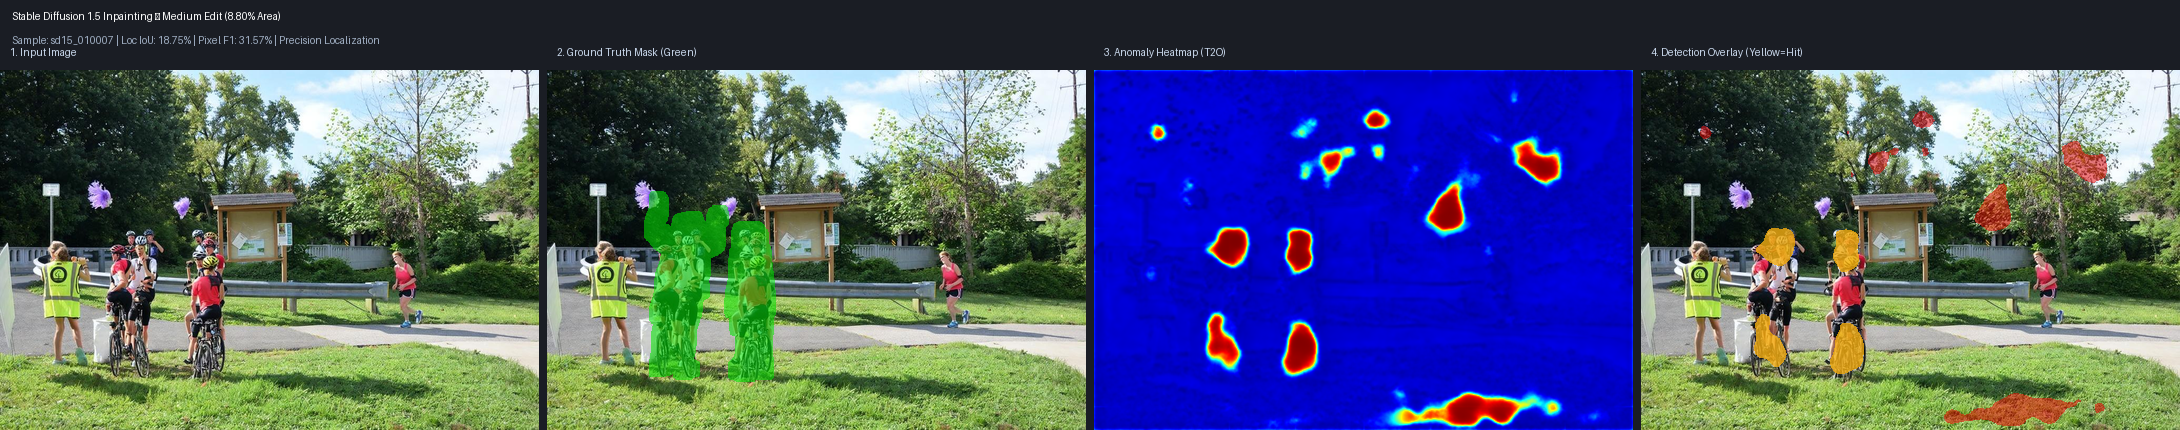
\includegraphics[width=\textwidth]{figures/sd15-localization.png}
\caption{SD1.5 development example from the earlier T2O diagnostic, sample sd15\_010007. From left to right, input image, reference region in green, anomaly heatmap, and predicted regions. Yellow indicates overlap with the reference and red marks predictions outside it.}
\Description{An outdoor scene shown with the reference edit, anomaly heatmap, and prediction overlay. The detector identifies portions of the edited figures and several genuine background regions.}
\label{fig:sd15-qual}
\end{figure*}

\begin{figure*}[t]
\centering
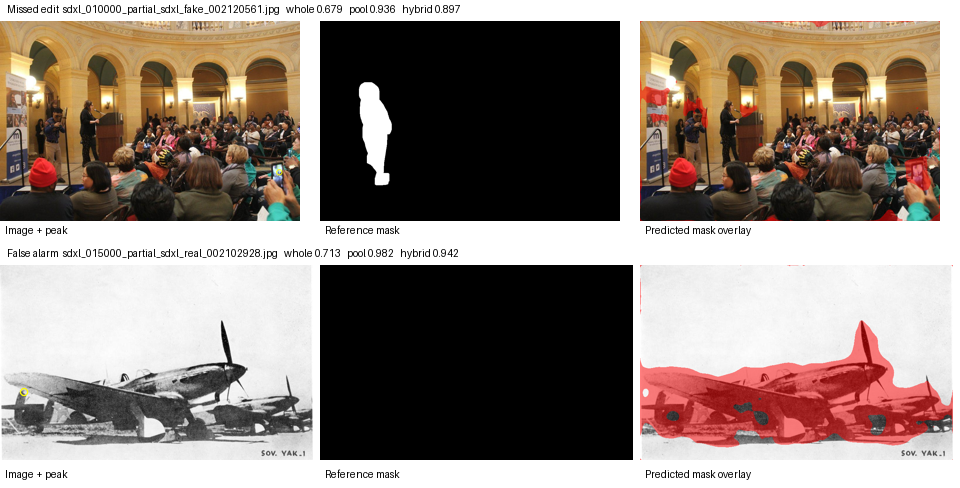
\includegraphics[width=\textwidth]{figures/sdxl-error-examples.png}
\caption{Two selected cases from the earlier SDXL error audit. The top row is a missed edit and the bottom row is a false alarm on a genuine image. Each row shows the input with its peak response marked, the reference mask, and the predicted region in red.}
\Description{Two rows with three panels each show a missed edit in an indoor scene and a false alarm on a genuine aircraft photograph. The genuine photograph has an empty reference mask.}
\label{fig:sdxl-errors}
\end{figure*}

\subsection{Published benchmark context}

Table~\ref{tab:published-context} places the work alongside prior approaches. All figures are taken from the common OpenSDID evaluation reported by FUSED~\cite{fused}. That evaluation trains on SD~1.5 and reports results across five editor groups. We list the publication venue of each method separately from the source of the measurements. A direct comparison with our development runs requires matched training exposure, split, scoring, and metric aggregation.

\begin{table}[t]
\caption{Selected literature scores from the common OpenSDID evaluation in FUSED~\cite{fused}. All scores are percentages. A dash denotes localization results unavailable in the cited table.}
\label{tab:published-context}
\centering
\small
\setlength{\tabcolsep}{3.5pt}
\begin{tabular}{@{}llrrr@{}}
\toprule
Method & Original venue & Acc. & Img. F1 & IoU \\
\midrule
FUSED & arXiv 2026 & 89.5 & 88.0 & 44.5 \\
MaskCLIP & CVPR 2025 & 82.0 & 77.8 & 42.7 \\
RINE & ECCV 2024 & 80.3 & 76.0 & -- \\
PSCC-Net & IEEE TCSVT 2022 & 76.8 & 68.0 & 29.7 \\
NPR & CVPR 2024 & 76.4 & 74.9 & -- \\
CAT-Net & IJCV 2022 & 76.2 & 65.6 & 37.4 \\
UniFD & CVPR 2023 & 75.7 & 72.2 & -- \\
MVSS-Net & IEEE TPAMI 2023 & 75.1 & 64.6 & 29.8 \\
DeCLIP & WACV 2025 & 73.1 & 71.4 & 25.2 \\
GramNet & CVPR 2020 & 72.3 & 67.2 & -- \\
CNNDetection & CVPR 2020 & 70.9 & 61.6 & -- \\
TruFor & CVPR 2023 & 69.8 & 58.6 & 36.9 \\
ObjectFormer & CVPR 2022 & 66.3 & 54.8 & 24.1 \\
FreqNet & AAAI 2024 & 66.3 & 56.4 & -- \\
IML-ViT & arXiv 2023 & 56.4 & 53.6 & 32.5 \\
\bottomrule
\end{tabular}
\end{table}

\section{Discussion, Limitations, and Future Work}

\subsection{Run provenance and comparison conditions}

\paragraph{Training budget.} The reported 10K configuration differs from the portable Kaggle notebook and dataset bundle. The notebook in the project uses a global batch of four and the bundle contains 1,640 training images. The 10K run manifest and training log are needed to link the reported settings to a checkpoint.

\paragraph{Pixel supervision.} The existing segmentation objective adds balanced binary cross-entropy and soft Dice loss. The balanced term averages foreground and background losses separately when both classes are present. Dice encourages overlap with the reference mask and is related to IoU. We will compare the combined loss with balanced cross-entropy alone at the same data and training budget, reporting overall and small-edit IoU.

\paragraph{Genuine-image rejection.} The joint-view model reached 84\% specificity at its selected operating point, compared with 74\% for the earlier Base model, while edited-image recall declined from 54\% to 34\%. The difference between mean genuine and edited scores increased, but whole-image AUROC fell from 0.6872 to 0.6450. We will test whether adding genuine images with difficult textures improves recall at a fixed false-positive rate. Specificity, recall, and overall accuracy will be reported together.

\paragraph{Inference.} The recorded ensemble uses weights of 0.15 for the whole-image score and 0.85 for the pooled local score. A 0.50/0.50 blend, tiles at multiple scales, and horizontal flips are separate inference choices. We will vary each on fixed checkpoints and choose settings on validation. Flip inference incurs an additional forward pass per flipped tile. Its effect on IoU and latency requires a matched comparison.

The 10K run summary and literature scores use different documented training conditions. A performance ranking requires a source-disjoint evaluation with matched training exposure, split, decision rules, and metric aggregation.

The local experiments compare existing configurations with different training and scoring choices. They do not isolate the contribution of cross-attention, joint-view training, or flip augmentation. The repeatedly inspected development subset has limited statistical power, especially for the smallest edit bins. The reported results therefore support error analysis and experiment design. To assess generalization, we will fix the image and mask decision rules on validation data before evaluating on an independent source-group split. A separate controlled comparison will hold training data, initialization, and compute budget fixed while varying supervision or fusion.
